% Chapter Template
\chapter{Conclusiones} % Main chapter title
\label{Capitulo5} % Change X to a consecutive number; for referencing this chapter elsewhere, use \ref{ChapterX}
\lhead{\emph{Conclusiones}}

%----------------------------------------------------------------------------------------
%	SECTION 1
%----------------------------------------------------------------------------------------
Mediante la utilización Mosaico Bayer y método de Malvar (véa \ref{capMalvar}) previo a la generación de imágenes de cubo hiperespectral permite un filtrado que mejora detalles. 
Después de obtener ese resultado se aplica el método CTIS para obtener las imágenes y a dichas imágenes se le aplicamos el desenfoque (vea capítulo \ref{CapBlur}) y la nitidez (véa \ref{capSharpender}).
Posterior a ello se aplicaron las series de Daubichies (vea la sección \ref{rDau}) aunque no se noto alguna mejora significante por lo que se determinó dejar el procedimiento hasta la aplicación del desenfoque y la nitidez.

\begin{figure}[h]
\begin{center}$
\begin{array}{lll}
\subfloat[Original]{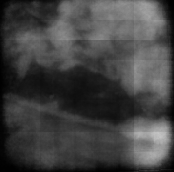
\includegraphics[scale=1.5]{./images/RESULTS/compare870/original.png}}&
\subfloat[MSB]{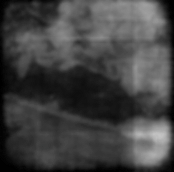
\includegraphics[scale=1.125]{./images/RESULTS/compare870/MSB.png}}
\end{array}$
\end{center}

\caption{Proceso para MSBD en extracción 870-845.}
\label{pics:process}
\end{figure}